\subsection{Przeprowadzić uczenie ostatniej warstwy splotowej wraz z częścią
klasyfikującą}

Ostatnią warstwą splotową w sieci EfficientNetB0 jest warstwa top\_conv, która jest trzecią warstwą od góry. Z tego powodu zamrożono wszystkie warstwy sieci poza trzema ostatnimi. Jako wagi początkowe zastosowano wagi imagenet. Następnie przeprowadzono uczenie z wykorzystaniem zbioru treningowego. W trakcie uczenia zastosowano optymalizator Adam, funkcję straty sparse categorical crossentropy oraz metrykę accuracy. Przetestowano różne wartości współczynnika uczenia, ostatecznie wybrano wartość 1e-5. Po 40 epokach uczenia osiągnięto na zbiorze testowym \textbf{accuracy na poziomie 0.74, loss na poziomie 0.66} oraz macierz pomyłek przedstawioną w tabeli \ref{tab:z2a}. Wyniki uczenia w czasie przedstawiono na rysunku \ref{fig:z2a}. Dalsze uczenie nie przynosiło poprawy wyników.

% Confusion Matrix:
%  [[ 32  18  29  49]
%  [  0 229   4   1]
%  [  1   4 105   1]
%  [  4  19  24  76]]

% \begin{table}[H]
% \centering
% \begin{tabular}{|c|c|c|c|c|}
% \hline
% klasa & 0 & 1 & 2 & 3 \\ \hline
% 0 & 32 & 18 & 29 & 49 \\ \hline
% 1 & 0 & 229 & 4 & 1 \\ \hline
% 2 & 1 & 4 & 105 & 1 \\ \hline
% 3 & 4 & 19 & 24 & 76 \\ \hline
% \end{tabular}
% \caption{Macierz pomyłek dla zadania 2a}
% \label{tab:z2a}
% \end{table}

\begin{table}[ht]
\centering
\begin{tabular}{|l|c|c|c|c|}
\hline
Przewidywane: & \textbf{samolot (0)} & \textbf{dron (1)} & \textbf{helikopter (2)} & \textbf{ptak (3)} \\ \hline
\textbf{samolot (0)} & 32 & 18 & 29 & 49 \\ \hline
\textbf{dron (1)} & 0 & 229 & 4 & 1 \\ \hline
\textbf{helikopter (2)} & 1 & 4 & 105 & 1 \\ \hline
\textbf{ptak (3)} & 4 & 19 & 24 & 76 \\ \hline
\end{tabular}
\caption{Macierz pomyłek dla zadania 2a}
\label{tab:z2a}
\end{table}
    

\begin{figure}[H]
    \centering
    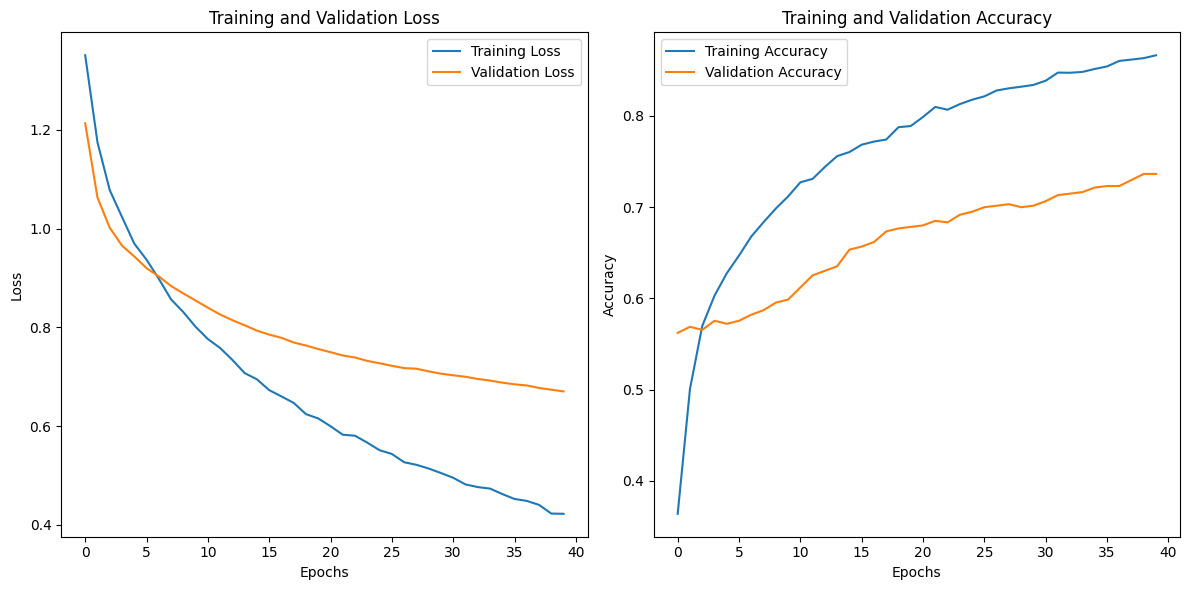
\includegraphics[width=0.8\textwidth]{img/z2a.png}
    \caption{Wyniki uczenia dla zadania 2a}
    \label{fig:z2a}
\end{figure}


Model bardzo dobrze radzi sobie z wykrywaniem dronów, za to ma problem z wykrywaniem samolotów.



%ile parametrów trainable

\subsection{Wytrenować całą sieć dla zadanych danych}
W tym zadaniu odmrożono wszystkie warstwy EfficientNetB0 i nadano im wagi początkowe imagenet. Następnie przeprowadzono uczenie z wykorzystaniem zbioru treningowego. W trakcie uczenia zastosowano optymalizator Adam, funkcję straty sparse categorical crossentropy oraz metrykę accuracy. Przetestowano różne wartości współczynnika uczenia, ostatecznie wybrano wartość 1e-5. Podczas uczenia zastosowano mechanizm early stopping, który zatrzymywał uczenie jeśli przez 4 epoki nie następowała poprawa wyników. Uczenie zatrzymało się po 22 epokach. Ostatecznie osiągnięto na zbiorze testowym \textbf{accuracy na poziomie 0.63, loss na poziomie 1.01} oraz macierz pomyłek przedstawioną w tabeli \ref{tab:z2b}. Wyniki uczenia w czasie przedstawiono na rysunku \ref{fig:z2b_with_w}.

% Test loss: 1.0159192085266113, Test accuracy: 0.6325503587722778
% Confusion Matrix:
%  [[ 56  17  55   0]
%  [  0 234   0   0]
%  [ 22   1  87   1]
%  [  9  36  78   0]]

% \begin{table}[H]
% \centering
% \begin{tabular}{|c|c|c|c|c|}
% \hline
% klasa  & 0 & 1 & 2 & 3 \\ \hline
% 0 & 56 & 17 & 55 & 0 \\ \hline
% 1 & 0 & 234 & 0 & 0 \\ \hline
% 2 & 22 & 1 & 87 & 1 \\ \hline
% 3 & 9 & 36 & 78 & 0 \\ \hline
% \end{tabular}
% \caption{Macierz pomyłek dla zadania 2b z wagami imagenet}
% \label{tab:z2b}
% \end{table}

\begin{table}[ht]
\centering
\begin{tabular}{|l|c|c|c|c|}
\hline
Przewidywane: & \textbf{samolot (0)} & \textbf{dron (1)} & \textbf{helikopter (2)} & \textbf{ptak (3)} \\ \hline
\textbf{samolot (0)} & 56 & 17 & 55 & 0 \\ \hline
\textbf{dron (1)} & 0 & 234 & 0 & 0 \\ \hline
\textbf{helikopter (2)} & 22 & 1 & 87 & 1 \\ \hline
\textbf{ptak (3)} & 9 & 36 & 78 & 0 \\ \hline
\end{tabular}
\caption{Macierz pomyłek dla zadania 2b z wagami początkowymi imagenet}
\label{tab:z2b}
\end{table}
    
    
\begin{figure}[H]
    \centering
    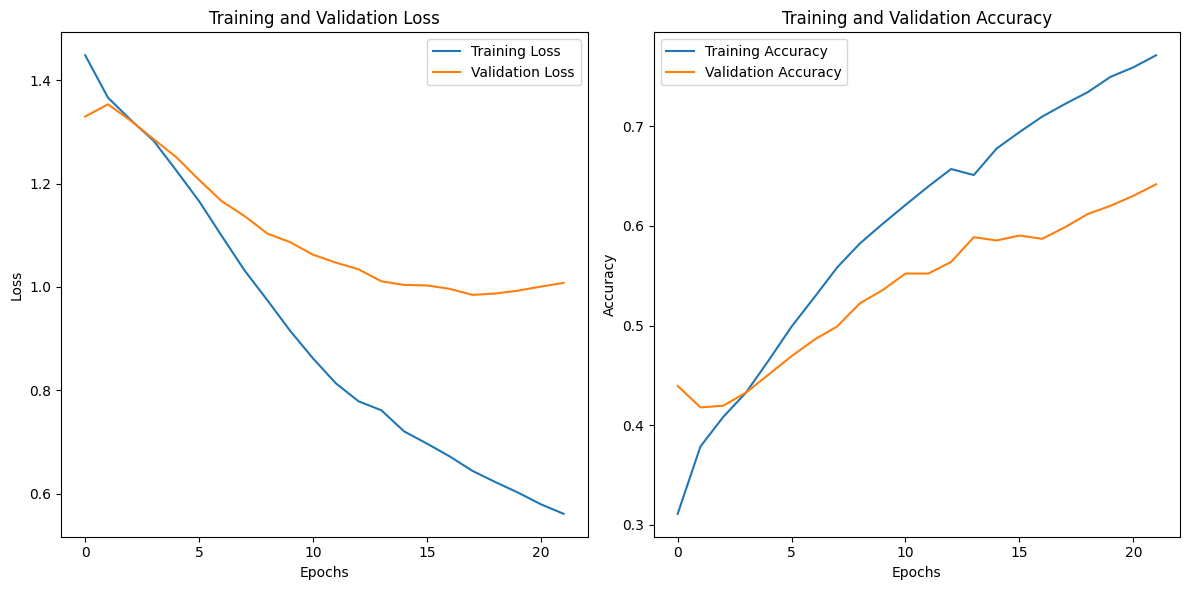
\includegraphics[width=0.8\textwidth]{img/z2b_with_w.png}
    \caption{Wyniki uczenia dla zadania 2b z wagami imagenet}
    \label{fig:z2b_with_w}
\end{figure}

Model bardzo dobrze radzi sobie z wykrywaniem dronów (100\% dronów zostało wykrytych), za to ma problem z wykrywaniem samolotów i ptaków - są one klasyfikowane jako helikoptery. Przykładowe błędne detekcje przedstawiono na rysunku \ref{fig:z2b_imgs}.

\begin{figure}[H]
    \centering
    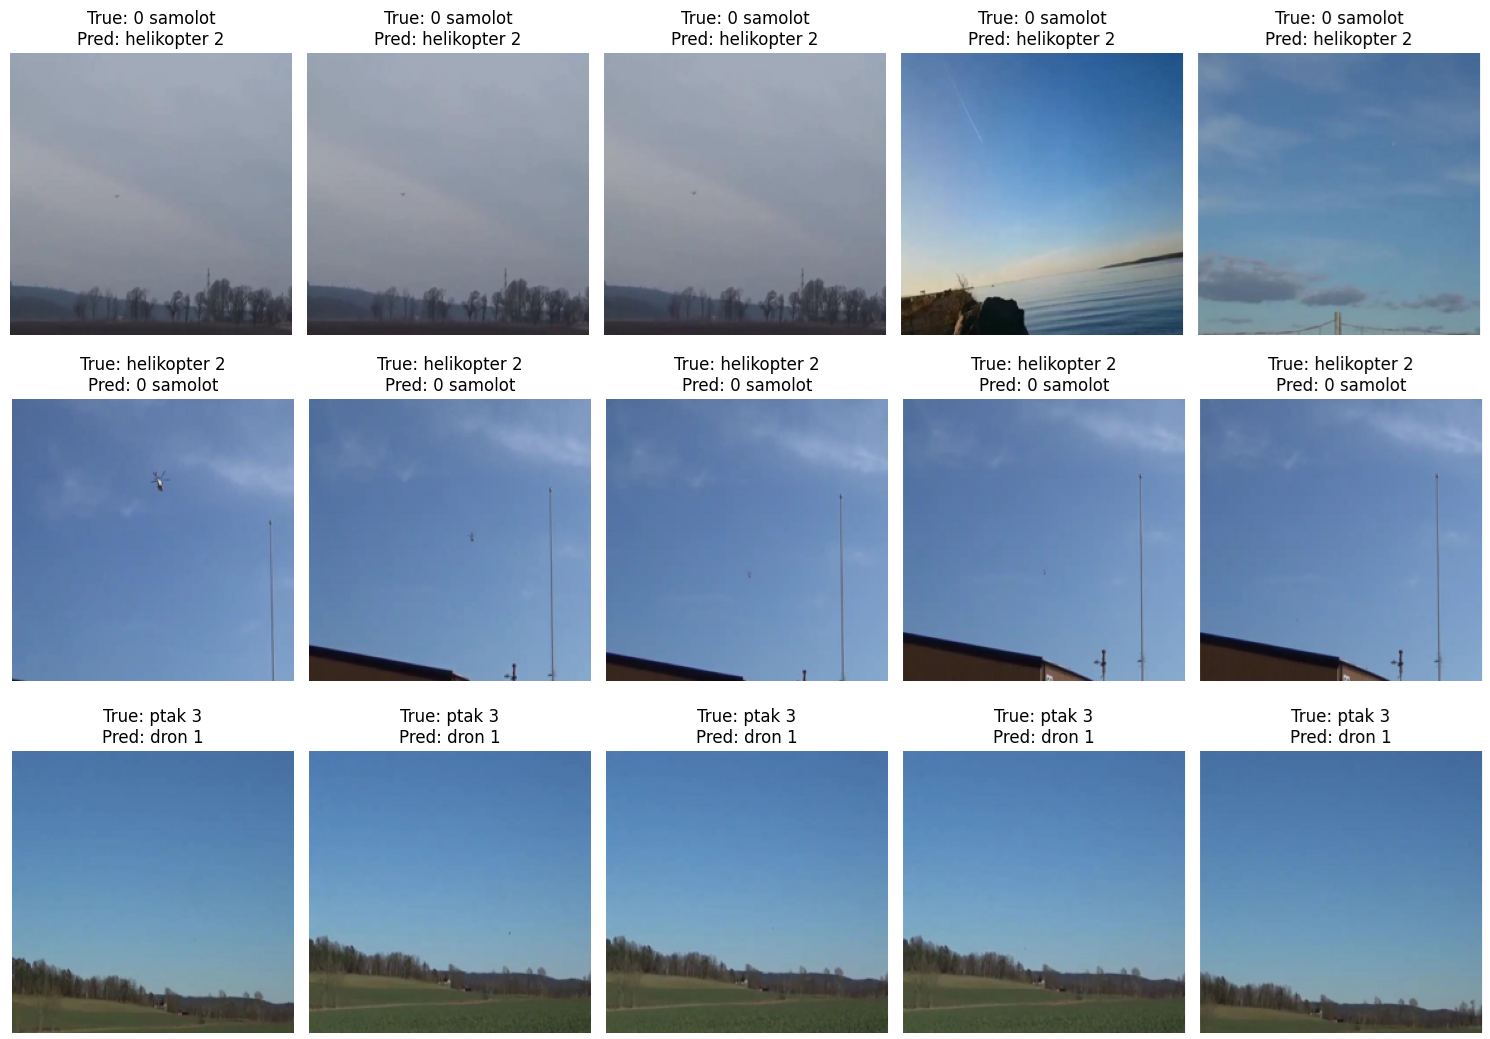
\includegraphics[width=0.8\textwidth]{img/z2b_imgs.png}
    \caption{Przykładowe błędne detekcje}
    \label{fig:z2b_imgs}
\end{figure}


Próbowano także wytrenować całą sieć bez zadanych wag początkowych, jednak w tym przypadku wyniki były dużo gorsze (accuracy na poziomie 0.38). Może to wynikać z faktu, że zbiór treningowy jest stosunkowo mały, a wagi początkowe z imagenet są lepsze niż losowe.

\subsection{Uprościć strukturę sieci wytrenowanej w zadaniu 2b (np. poprzez usunięcie jednej lub więcej końcowych warstw splotowych, usunięcie warstw regularyzujących itp.) i ponowić uczenie}

W celu uproszczenia sieci usunięto wszystkie warstwy EfficientNetB0 powyżej warstwy block5b\_add oraz zmodyfikowano head. Początkowo model miał 4,012,672 (15.31 MB) trainable params oraz 42,023 (164.16 KB) non-trainable params. Po uproszczeniu wielkość zmalała do 703,144 (2.68 MB) trainable params oraz 13,255 (51.78 KB) non-trainable params. Następnie przeprowadzono uczenie z wykorzystaniem zbioru treningowego. W trakcie uczenia zastosowano optymalizator Adam z współczynnikiem uczenia 1e-5, funkcję straty sparse categorical crossentropy oraz metrykę accuracy. Po 20 epokach osiągnięto na zbiorze testowym \textbf{accuracy na poziomie 0.52, loss na poziomie 1.18} oraz macierz pomyłek przedstawioną w tabeli \ref{tab:z2c}. Wyniki uczenia w~czasie przedstawiono na rysunku \ref{fig:z2c}.

% Confusion Matrix:
%  [[  6  25  60  37]
%  [  0 175  52   7]
%  [  2   5  99   5]
%  [  6   7  80  30]]

\begin{table}[ht]
\centering
\begin{tabular}{|l|c|c|c|c|}
\hline
Przewidywane: & \textbf{samolot (0)} & \textbf{dron (1)} & \textbf{helikopter (2)} & \textbf{ptak (3)} \\ \hline
\textbf{samolot (0)} & 6 & 25 & 60 & 37 \\ \hline
\textbf{dron (1)} & 0 & 175 & 52 & 7 \\ \hline
\textbf{helikopter (2)} & 2 & 5 & 99 & 5 \\ \hline
\textbf{ptak (3)} & 6 & 7 & 80 & 30 \\ \hline
\end{tabular}
\caption{Macierz pomyłek dla zadania 2c}
\label{tab:z2c}
\end{table}

\begin{figure}[H]
    \centering
    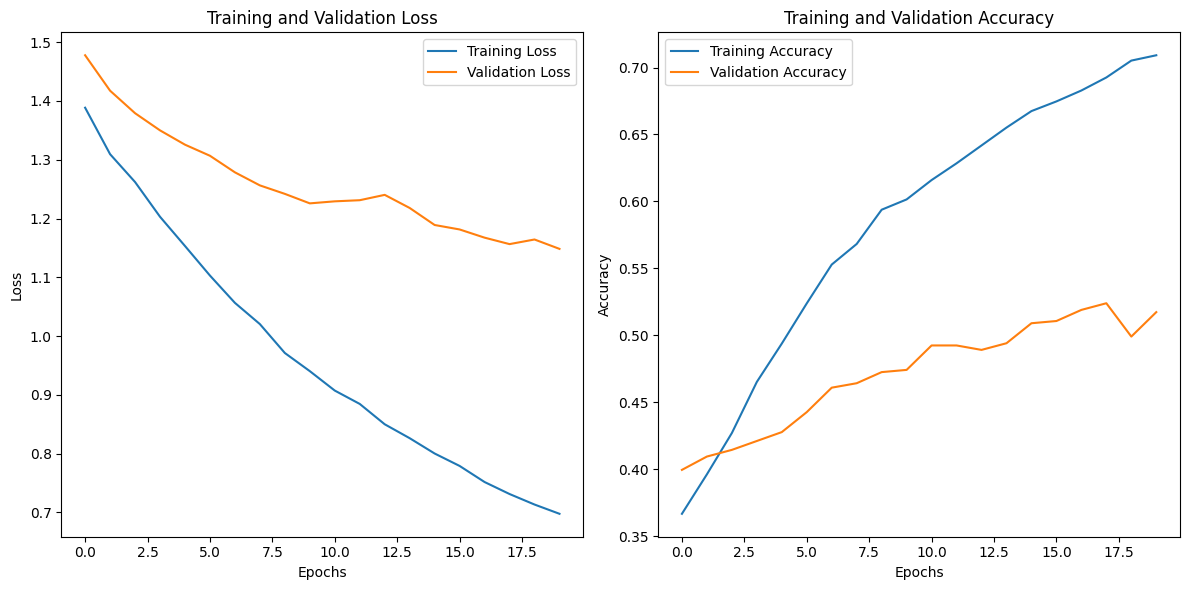
\includegraphics[width=0.8\textwidth]{img/z2c.png}
    \caption{Wyniki uczenia dla zadania 2c}
    \label{fig:z2c}
\end{figure}

\subsection{Zanalizować wyniki 2 abc}
Uczenie ostatniej warstwy splotowej pozwoliło osiągnąć dokładność 74\%, co jest średnio zadowalającym wynikiem. Jednak, jeśli wystarczyłaby nam informacja binarna (jest dron / nie ma drona), to taki klasyfikator mógłby być użyteczny, ponieważ 97,96\% dronów zostało wykrytych i jedynie 11,32\% nie-dronów zostało sklasyfikowanych jako drony. Uczenie całej sieci z wagami imagenet pozwoliło osiągnąć dokładność 63\%, co jest wynikiem gorszym niż w przypadku uczenia ostatniej warstwy splotowej, jednak w tym przypadku 100\% dronów ze zbioru testowego ostało poprawnie wykrytych. Uproszczenie sieci pozwoliło zmniejszyć wielkość modelu oraz liczbę parametrów ponad 5-krotnie, jednak kosztem dokładności - wynik wyniósł zaledwie 52\%. Warto zauważyć, że w przypadku uproszczenia sieci, model nadal całkiem dobrze radzi sobie z wykrywaniem dronów (75\% dronów zostało wykrytych), jednak ma problem z wykrywaniem pozostałych klas.

Wyniki nie są dość zadowalające, aby móc wykorzystać model do praktycznych zastosowań. Możliwe przyczyny niskiej dokładności to mała ilość danych treningowych oraz ich jakość. Przykład słabej jakości danych widać na rysunku \ref{fig:z2b_imgs} - nawet człowiek ma problem z klasyfikacją niektórych obrazów. 